\documentclass[11pt]{article}

% ---------------------------------------------------------------------------
% From Shor breaking secp256k1 to the point-add challenge -- a background
% overview meant to lay out the relevant context (in preparation for writing).
% Self-contained.
% Build: make   (internally uses xelatex; English-only, article class)
% ---------------------------------------------------------------------------

\usepackage[margin=1in]{geometry}
\usepackage{amsmath,amssymb}
\usepackage{booktabs}
\usepackage{array}
\usepackage{xcolor}
\usepackage{listings}
\usepackage{enumitem}
\usepackage{pifont}
\usepackage{tikz}
\usepackage{hyperref}
\hypersetup{
  colorlinks=true,
  allcolors={[HTML]{1A5FB4}},
  linktoc=all,
}
% Make the whole "\S N" (including the \S sign) one clickable link jumping to the section
\newcommand{\secref}[1]{\hyperref[#1]{\S\ref*{#1}}}

\definecolor{codebg}{gray}{0.96}
\lstset{
  basicstyle=\ttfamily\small,
  backgroundcolor=\color{codebg},
  breaklines=true,
  columns=fullflexible,
  frame=single,
  framesep=4pt,
  xleftmargin=4pt,
  showstringspaces=false,
}
\let\c\lstinline

\newcommand{\cmark}{\ding{51}}
\newcommand{\xmark}{\ding{55}}
% Typeset code paths / identifiers: use the url mechanism so underscores/asterisks
% print verbatim and lines can break at / and .
\usepackage{url}
\DeclareUrlCommand\code{\urlstyle{tt}}
% Allow \code to break long identifiers at _ / . - (tt urlstyle otherwise won't
% break at underscores, overflowing tokens like weierstrass_elliptic_curve.rs).
\Urlmuskip=0mu plus 1mu\relax
\makeatletter
\g@addto@macro\UrlBreaks{\do\_\do\/\do\.\do\-}
\makeatother

\title{\textbf{From Shor Breaking secp256k1 to the Point-Add Challenge\\
\large Principles, Scoring Motivation, and Implementation Mapping---A Background Overview}}
\author{BenHuang2025 @ Brevis}
\date{2026-07-05}

\begin{document}
\maketitle

\begin{abstract}
This document lays out both the attack principle and the challenge background as groundwork for further writing, in two parts. \textbf{Part~I (General Principles)} explains \emph{how} Shor's algorithm step by step breaks the
elliptic-curve discrete logarithm (ECDLP) on secp256k1: from the problem reduction, the algorithm's steps, and the circuit framework, to the step-by-step evolution of the quantum state and the recovery of the private key after measurement. \textbf{Part~II (Implementation)} maps this
general theory onto the actual secp256k1 point-add challenge\footnote{Challenge site: \url{https://www.ecdsa.fail/}.}: which part of it the challenge actually implements, what scoring and verification rules it obeys, why almost the entire cost of the attack concentrates on the \textbf{elliptic-curve point addition} and the optimization focus in turn falls \emph{chiefly} on the \textbf{modular inverse (GCD)} inside it (with the surrounding field arithmetic a secondary but still live source of gains), and which file and function each section lands in.
To understand "why/how Shor breaks ECDLP," start with \textbf{Part~I} (\S1--\S7); to quickly align on "what this challenge is optimizing and what constraints it has,"
read \textbf{Part~II} (\S8--\S11) directly. The two parts are mutually independent and can be used as needed.
\end{abstract}

\tableofcontents

% #####################################################################
\part{General Principles: How Shor Breaks ECDLP}
% #####################################################################

This part focuses on one thing---how Shor's algorithm turns the "classically hard problem" of recovering the private key into a computation a quantum machine can carry out efficiently. It is an
as-self-contained-as-possible background overview: after reading it you should be able to \emph{derive} how the private key is computed step by step, understand each step's
quantum state and the origin of each constructive/destructive interference, and know the exact position within the whole pipeline of the point-add primitive this challenge optimizes. As for \emph{the concrete optimization of that circuit},
that belongs to the engineering pipeline and is not covered here.

\paragraph{Notation used throughout.}
$E/\mathbb{F}_p$ is the secp256k1 curve, $p$ its 256-bit prime field characteristic, $\mathcal{O}$ the point at infinity (group identity);
$P$ is the base point, of prime order $r$, so the cyclic subgroup $\langle P\rangle\cong\mathbb{Z}_r$; the public key is $Q=kP$, the private key
$k\in\{1,\dots,r-1\}$ is the attack target; $n=256$ is the scalar bit width. The two quantum input registers hold $t$ bits each (i.e.\ $t$ qubits each), $M=2^{t}\gtrsim r$ is the quantum Fourier
transform (QFT) modulus, $\omega_M=e^{2\pi i/M}$, $\omega_r=e^{2\pi i/r}$. $\mathbb{Z}_N=\{0,\dots,N-1\}$
denotes the residues mod $N$. (Reminder: the public key is written $Q$, the QFT modulus is written $M$, so the two no longer share a single letter---this is the only departure from many textbooks' notation.)

% =====================================================================
\section{Challenge Overview}
\label{sec:overview}
% =====================================================================

\subsection{secp256k1 and its elliptic-curve group}

secp256k1 is the elliptic curve used by Bitcoin, Ethereum, and a great deal of TLS/signature machinery, defined over the prime field $\mathbb{F}_p$:
\[
E:\;y^2 = x^3 + 7 \pmod p,\qquad p = 2^{256}-2^{32}-977 .
\]
The affine points $(x,y)$ on the curve, together with a point at infinity $\mathcal{O}$, form an \textbf{abelian group} under the "chord-and-tangent" addition law, with $\mathcal{O}$
as identity. For two points $P_1=(x_1,y_1)$, $P_2=(x_2,y_2)$ (with $P_1\neq\pm P_2$), their sum $P_3=(x_3,y_3)=P_1+P_2$ is given by
\begin{equation}
\lambda=\frac{y_2-y_1}{x_2-x_1},\qquad x_3=\lambda^2-x_1-x_2,\qquad y_3=\lambda(x_1-x_3)-y_1
\label{eq:padd}
\end{equation}
(for point doubling $P_1=P_2$ use $\lambda=\tfrac{3x_1^2}{2y_1}$ instead, since secp256k1's $a$-coefficient is $0$). All arithmetic here is in
$\mathbb{F}_p$; note that \eqref{eq:padd} contains one division $(x_2-x_1)^{-1}$---i.e.\ one \emph{modular inverse},
which will be the most expensive part of the point-add circuit later (\secref{ssec:inv}).

The order of the base point $P$ is a 256-bit prime $r$ (secp256k1's cofactor is $1$, so the whole curve group is $\langle P\rangle\cong\mathbb{Z}_r$).
\textbf{Scalar multiplication} $k\mapsto kP$ is adding $P$ to itself $k$ times; it is the basis of all ECC operations.

\subsection{The discrete logarithm problem (ECDLP) and its classical hardness}

The security of elliptic-curve cryptography rests on the \textbf{elliptic-curve discrete logarithm problem (ECDLP)}:
\begin{center}
\emph{given the base point $P$ and the public key $Q=kP$, find the scalar $k$.}
\end{center}
The forward direction $k\mapsto kP$ takes only $\mathcal{O}(n)$ point additions via double-and-add, at little cost; but the reverse, recovering $k$ from $Q$, takes even the best \emph{classical}
algorithms (Pollard $\rho$ / baby-step giant-step) $\Theta(\sqrt r)\approx 2^{128}$ group operations---utterly infeasible when $r\approx 2^{256}$.
This is precisely the foundation of ECDSA's unforgeability: forging a signature is equivalent to solving this ECDLP.

The significance of Shor's algorithm is that a sufficiently large \emph{fault-tolerant} quantum computer can solve for $k$ in
\textbf{polynomial time} $\mathrm{poly}(n)$ in the scalar bit width, breaking through the $2^{128}$ classical wall. The following sections lay out the principles of this quantum algorithm.

\subsection{The primitive this challenge optimizes, and the roadmap of this part}

The circuit \href{https://ecdsa.fail}{ecdsa.fail} asks you to optimize is exactly the \textbf{innermost primitive} used when attacking ECDLP with Shor's algorithm:
on a quantum superposition, controllably and reversibly adding a \emph{classical} point to a curve point. It is this one because the entire attack can be summarized in a single sentence:
\begin{center}
\emph{the total quantum arithmetic of the attack} $\;\approx\;$ \emph{one elliptic-curve point addition} $\;\times\;\mathcal{O}(n)$ \emph{calls}.
\end{center}
This part then unfolds that sentence layer by layer following Shor's flow: first reduce ECDLP to "find a hidden structure" (\secref{sec:reduce}), list the algorithm's steps
(\secref{sec:steps}), draw the circuit framework and locate the primitive (\secref{sec:circuit}), then derive the quantum evolution and interference state by state
(\secref{sec:evolve}), and finally explain how, after measurement, $k$ is recovered and \emph{confirmed} (\secref{sec:period}).

% =====================================================================
\section{How the problem moves over to the quantum side}
\label{sec:reduce}
% =====================================================================

This section involves no abstract framework; it settles just one concrete thing---how the number-theoretic problem "given $P$, $Q$ on the curve, find the $k$ with $Q=kP$" gets step by step
encoded into the preparation and measurement of a quantum state. The whole conversion is the following four steps.

\subsection{Step one: choose a probe function that "hides $k$ in a period"}

What we know is a set of \emph{classical} data: the curve parameters ($p$, base point $P$, order $r$) and a public-key point $Q$; the unknown is $k$. Classically, this is a search in a space of size
$r\approx2^{256}$, infeasible. The first step of the conversion is to not solve for $k$ directly, but construct a "probe function":
\begin{equation}
f(a,b)\;=\;aP+bQ\;=\;aP+b(kP)\;=\;(a+kb)\,P,\qquad a,b\in\mathbb{Z} .
\label{eq:f}
\end{equation}
Along the way we use $Q=kP$---$P,Q$ are known constants, and $a,b$ are freely chosen inputs. The key is the \textbf{symmetry} of $f$: shifting the input along the vector
$(-k,1)$ leaves the value of $f$ \emph{unchanged},
\begin{equation}
f(a-k,\ b+1)=\bigl((a-k)+k(b+1)\bigr)P=(a+kb)\,P=f(a,b),
\label{eq:period}
\end{equation}
and more generally $f(a,b)=f(a',b')\iff (a-a')+k(b-b')\equiv0\pmod r$. In other words, the private key $k$ has been encoded as the
"period direction / slope" $(-k,1)$ of $f$---finding this period direction is the same as reading out $k$. At this point, "compute the discrete log" has been rewritten as "find the
period of a function." (Readers familiar with the abstract theory will recognize this as a two-dimensional instance of the abelian hidden subgroup problem; but the four steps below are all we need, with no need to unpack it.)

\subsection{Step two: pack $a,b$ and the curve point into qubits}

To "find the period" on a quantum machine, first encode all the objects in \eqref{eq:f} into qubits:
\begin{itemize}[leftmargin=1.4em]
\item \textbf{Two input registers} (call them the $a$ register and the $b$ register): $t$ qubits each ($t\approx n=256$; we write "$\approx$" because $r$ is not a power of $2$, we only need $2^t\gtrsim r$, and the exact value has a few bits of slack---see \secref{sec:steps} and \secref{ssec:cf}), holding the binary representation of scalars $a$, $b$ respectively.
\item \textbf{One point register}: a curve point is represented by its two $\mathbb{F}_p$ coordinates $(x,y)$, each a 256-bit field element, so about
$2\times256$ data qubits (plus a handful of ancilla for carries / the coordinate system).
\end{itemize}
Here two concepts must be kept apart: a \textbf{register} is a \emph{group of physical qubits} (hardware, a "container"); whereas the ket $\lvert a\rangle$ denotes the
$a$ register being in the \emph{computational basis state} that "encodes the integer $a$" (it has $2^t$ basis states, one per $a\in\{0,\dots,2^t-1\}$), and $\lvert(x,y)\rangle$
likewise means the point register encodes the point $(x,y)$. So a computational basis state $\lvert a\rangle\lvert b\rangle\lvert (x,y)\rangle$
is nothing but three bit strings---but once the algorithm runs, these registers are usually in a \emph{superposition} of basis states (e.g.\ the $a$ register in
$\tfrac{1}{\sqrt{2^t}}\sum_a\lvert a\rangle$), no longer a single $\lvert a\rangle$ (the rigorous state evolution is in \secref{sec:evolve}).
The classical probe function $f$ is then realized as a \textbf{reversible circuit} $U_f$ acting on these qubits: $\lvert a,b\rangle\lvert\mathcal{O}\rangle\mapsto
\lvert a,b\rangle\lvert aP+bQ\rangle$ (its construction is in \secref{sec:circuit}).

\subsection{Step three: turn "search for $k$" into "prepare a superposition carrying the $k$-period"}

With $U_f$ in hand, the core step of the conversion is: rather than trying $(a,b)$ one by one, first prepare all $(a,b)$ into a \emph{superposition}, then evaluate $f$
on the whole superposition at once.
\begin{enumerate}[leftmargin=1.9em]
\item Apply one layer of $H$ to each input register (each qubit becomes $\tfrac{1}{\sqrt2}(\lvert0\rangle+\lvert1\rangle)$). This $H$
step, \emph{in one shot}, puts both registers \emph{simultaneously} into a uniform superposition over all $M^2$ basis states $\lvert a,b\rangle$ ($M=2^t$):
\[
\frac{1}{M}\sum_{a,b=0}^{M-1}\lvert a,b\rangle\,\lvert\mathcal{O}\rangle .
\]
\item Apply $U_f$ \emph{once}. Because quantum evolution is \emph{linear}, $U_f$ acts on \emph{every term} of the sum---so a single application evaluates $f$ on all
$M^2$ inputs at once:
\[
\frac{1}{M}\sum_{a,b=0}^{M-1}\lvert a,b\rangle\,\lvert\mathcal{O}\rangle
\;\xrightarrow{\;U_f\;}\;
\frac{1}{M}\sum_{a,b=0}^{M-1}\lvert a,b\rangle\,\lvert aP+bQ\rangle .
\]
\end{enumerate}
\paragraph{This step is the very essence of quantum computing ("superposition" $\neq$ "enumeration").}
This deserves a close look, especially to clarify that the sum $\sum_{a,b}$ above is \emph{not} a classical "iteration." Here $a,b$ are each $t$ bits,
taking values only in $\{0,\dots,M-1\}$ ($M=2^t$, \emph{finite}, not the unbounded integers), $M^2$ pairs in all. For a classical machine to actually compute $f$ at all these $M^2$ pairs $(a,b)$,
it would have to evaluate it $M^2=2^{512}$ times \emph{one by one}---completely impossible. The quantum effect \emph{looks} the same (the values of $f$ at all $(a,b)$ are already
obtained), yet there is no one-by-one evaluation loop:
\begin{itemize}[leftmargin=1.4em]
\item \textbf{Superposition} encodes exponentially many branches into \emph{linearly} many qubits: one register of $t=256$ qubits, each passed through a single $H$ ($t$ gates in all), already generates
a superposition of $2^{256}$ $\lvert a\rangle$'s ($H^{\otimes t}\lvert0\rangle^{\otimes t}=\tfrac{1}{\sqrt M}\sum_a\lvert a\rangle$); the two registers together use $2t$ qubits and $2t$ gates for all $M^2$ pairs. These
$M^2$ pairs $(a,b)$ are not $M^2$ independent objects but amplitudes of \emph{one and the same} state vector.
\item \textbf{Quantum parallelism} makes \emph{one} application of $U_f$ (by linearity) act on all branches at once---one application encodes this \emph{entire lookup table}
of "input $\mapsto aP+bQ$" into the state.
\end{itemize}
So the qubit count and gate count throughout are $\mathrm{poly}(t)$, with no $2^t$ factor: some $t$-order qubits carry the computation of $2^{512}$ branches. The exponential
"width" exists only in the state vector and corresponds to no per-item operation---\emph{this is the fundamental difference of quantum from classical}.

But it must also be stressed: this is not a "free brute-force search." This table \emph{cannot be read out}---one measurement collapses to a single random $(a,b)$, and all other branches are lost.
So quantum parallelism \emph{by itself brings no speedup}. The real power comes next, from the \textbf{interference} of the QFT, which extracts from this "already-computed but not directly readable" table, \emph{in one shot},
a single \emph{global} property---the hidden period of $f$ (that is, the private key $k$; how the QFT singles it out is in step four and \secref{sec:evolve}). \textbf{Superposition $+$ parallelism $+$ interference}
together are the real source of Shor's speedup over classical; parallel preparation alone is not enough.

The result is an \textbf{entangled state}: the input $(a,b)$ is correlated with the point value $aP+bQ$, and by \eqref{eq:period} the whole state has $(-k,1)$ as its
\emph{hidden period}. An essential shift has happened here---classically solving for $k$ takes about $2^{128}$ evaluations, whereas the quantum machine does \emph{one} coherent evaluation and thereby completes the computation of $f$
on exponentially many inputs, and the periodicity of $k$ now physically exists in the structure of this state (the rigorous ket-by-ket evolution is in \secref{sec:evolve}).
The only expensive part is precisely this step's $U_f$ ($\approx2n$ point additions), i.e.\ the primitive this challenge optimizes.

\subsection{Step four: use the QFT to "read out" the period}

The hidden period already exists in the state, but \emph{direct} measurement only collapses randomly and cannot read it out. The last step is to first apply a QFT to each input register, letting \textbf{quantum
interference} turn the periodic structure into measurable peaks in the frequency domain, then measure the \emph{same pair} of registers. $\mathrm{QFT}_M$ is the discrete Fourier
transform over $\mathbb{Z}_M$; it maps the $a$ register to its \emph{Fourier conjugate variable} $c$ and $b$ to $d$---so $c,d$ live on the \textbf{same pair of registers} as $a,b$,
just switched from the "position basis" to the "frequency basis," and their values are not equal (just as the classical discrete Fourier transform sends a sequence $\{x_n\}$ to its spectrum $\{\hat x_k\}$: here
$c,d$ play the role of $\hat x_k$). The result is that the measured integer pair $(c,d)$ satisfies, with high probability,
\begin{equation}
d\;\equiv\;k\,c\pmod r,
\label{eq:readout}
\end{equation}
so as long as $c\not\equiv0$, $k\equiv d\,c^{-1}\pmod r$ follows in one step. At this point a classical number-theoretic problem has been fully converted into a quantum procedure:
\emph{encode $k$ as the period of $f$ $\to$ pack $f$ into qubits $\to$ use one reversible evaluation to pour the period into the superposition $\to$ read it out with the QFT}.
As for why the QFT can single out \eqref{eq:readout} and why the peaks fall exactly on this line, that is the interference derivation of \secref{sec:evolve}; how to recover and \emph{confirm} $k$ from $(c,d)$
is \secref{sec:period}.

% =====================================================================
\section{Execution Steps}
\label{sec:steps}
% =====================================================================

This section gives the panorama first. The whole algorithm is the following \textbf{five steps} (hereafter written \textbf{\hyperref[step:prep]{Step 1}} through \textbf{\hyperref[step:recover]{Step 5}}; when later sections say "\hyperref[step:eval]{Step 2}"
they mean \hyperref[step:eval]{Step 2} here); this section states the operator and register scale used by each step, leaving the mathematical unfolding to \secref{sec:evolve}--\secref{sec:period}.

\begin{enumerate}[label=\textbf{Step \arabic*.},leftmargin=3.8em,itemsep=3pt]
\item\label{step:prep} \textbf{Prepare the superposition.} The two $t$-bit input registers (the $a$ register, the $b$ register) each go through $H^{\otimes t}$, placing them in a uniform superposition over
$\{0,\dots,M-1\}$ ($M=2^t$); the point register is initialized to $\lvert\mathcal{O}\rangle$.
\item\label{step:eval} \textbf{Reversible evaluation of $f$ (this step is where all the cost lives).} Apply the unitary $U_f:\lvert a,b\rangle\lvert\mathcal{O}\rangle\mapsto
\lvert a,b\rangle\lvert aP+bQ\rangle$---\emph{internally it is two scalar multiplications, about $2n$ controlled elliptic-curve point additions}
(unfolded, with the primitive's location, in \secref{sec:circuit}). It almost monopolizes the whole machine's Toffoli and qubit budget, and is the
"\hyperref[step:eval]{Step 2}" referred to repeatedly below.
\item\label{step:qft} \textbf{Double QFT.} Apply $\mathrm{QFT}_M$ to \emph{each} of the $a$, $b$ input registers (relatively cheap, see \secref{ssec:qft}).
\item\label{step:measure} \textbf{Measure.} Measure the two input registers, obtaining an integer pair $(c,d)\in\{0,\dots,M-1\}^2$. (The point register may or may not be measured; it does not affect the result.)
\item\label{step:recover} \textbf{Classical recovery $+$ verification.} From $(c,d)$, via rounding/modular division, solve for a candidate $k$, and verify with $kP\stackrel{?}{=}Q$; on failure go back to Step 1
and resample (see \secref{sec:period}).
\end{enumerate}

\paragraph{The trade-off in register size.}
Ideally the two input registers would work directly over $\mathbb{Z}_r$ ($M=r$), making the interference "clean" (\secref{ssec:ideal}); but real
hardware register widths are powers of $2$, so take $M=2^t$ with $2^t\gtrsim r$ (usually $t\approx n$, and to raise the single-shot success rate one can go up to $\approx 2n$).
$M$ not being an integer multiple of $r$ brings "leakage," handled by the nearest-integer rounding of \secref{ssec:leak} and \secref{sec:period}. The whole algorithm's \textbf{cost
balance} is: \hyperref[step:eval]{Step 2}'s $\Theta(n)$ point additions, each containing several modular multiplications and \emph{one modular inverse}, dominate; Steps 1 and 3 use $\mathcal{O}(t)$ and
$\mathcal{O}(t^2)$ cheap gates respectively and are negligible. This is exactly why "optimizing the point-add primitive" deserves serious attention.

% =====================================================================
\section{Circuit Framework}
\label{sec:circuit}
% =====================================================================

\subsection{Registers and top-level structure}

Figure~\ref{fig:top} gives the top-level circuit---only the main structure, not down to the Toffoli level. The four registers from top to bottom are: two $t$-bit input
registers $a$, $b$; a \textbf{point register} initialized to $\lvert\mathcal{O}\rangle$ (in the circuit, a curve point is represented by its two
$\mathbb{F}_p$ coordinates, so about $2\times256$ data qubits, plus a few for carries/coordinate system); and a bundle of scratch/ancilla that must be cleared after use (\emph{ancilla / scratch qubits}; dashed in the figure, annotated as uncomputed back to $\lvert0\rangle$, reasoning in \secref{ssec:inv}). The whole $U_f$ (the reversible
evaluation of \hyperref[step:eval]{Step 2}) spans these wires.

\begin{figure}[h]
\centering
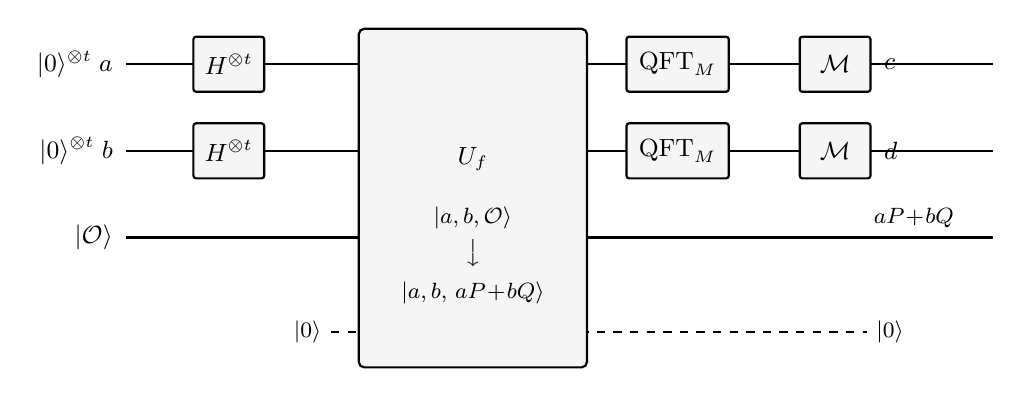
\begin{tikzpicture}[x=1cm,y=1cm,
  wire/.style={thick},
  gate/.style={draw,thick,fill=codebg,minimum height=7mm,minimum width=9mm,rounded corners=1pt,font=\small},
]
\def\ya{2.2}\def\yb{1.1}\def\yp{0}\def\ys{-1.2}
% register wires
\draw[wire] (0,\ya) -- (11,\ya);
\draw[wire] (0,\yb) -- (11,\yb);
\draw[wire] (0,\yp) -- (11,\yp);
\draw[wire,dashed] (2.6,\ys) -- (9.4,\ys);
% left labels
\node[left,font=\small] at (-0.05,\ya) {$\lvert 0\rangle^{\otimes t}\;a$};
\node[left,font=\small] at (-0.05,\yb) {$\lvert 0\rangle^{\otimes t}\;b$};
\node[left,font=\small] at (-0.05,\yp) {$\lvert \mathcal{O}\rangle$};
\node[left,font=\footnotesize] at (2.6,\ys) {$\lvert 0\rangle$};
% Hadamards
\node[gate] at (1.3,\ya) {$H^{\otimes t}$};
\node[gate] at (1.3,\yb) {$H^{\otimes t}$};
% U_f box
\node[draw,thick,fill=codebg,rounded corners=2pt,minimum width=2.9cm,minimum height=4.3cm] at (4.4,0.5) {};
\node[font=\small] at (4.4,1.0) {$U_f$};
\node[font=\footnotesize] at (4.4,0.25) {$\lvert a,b,\mathcal{O}\rangle$};
\node[font=\footnotesize] at (4.4,-0.2) {$\big\downarrow$};
\node[font=\footnotesize] at (4.4,-0.7) {$\lvert a,b,\,aP\!+\!bQ\rangle$};
% QFT
\node[gate,minimum width=13mm] at (7.0,\ya) {$\mathrm{QFT}_M$};
\node[gate,minimum width=13mm] at (7.0,\yb) {$\mathrm{QFT}_M$};
% measurement
\node[gate] at (9.0,\ya) {$\mathcal{M}$};
\node[gate] at (9.0,\yb) {$\mathcal{M}$};
\node[right,font=\small] at (9.5,\ya) {$c$};
\node[right,font=\small] at (9.5,\yb) {$d$};
\node[right,font=\footnotesize] at (9.4,\ys) {$\lvert 0\rangle$};
\node[above,font=\footnotesize] at (10.0,\yp) {$aP\!+\!bQ$};
\end{tikzpicture}
\caption{Top-level circuit framework. $H^{\otimes t}$ prepares the superposition; $U_f$ reversibly writes $aP+bQ$ into the point register (scratch cleared after use);
after the double $\mathrm{QFT}_M$, measuring the input registers gives $(c,d)$. The internal expansion of $U_f$ is in Figure~\ref{fig:oracle}.}
\label{fig:top}
\end{figure}

\subsection{Inside $U_f$: scalar mult $\to$ double-and-add $\to$ controlled point-add}

The $aP$, $bQ$ that $U_f$ must compute are both \textbf{scalar multiplications}. Expanding the scalar in binary $a=\sum_{i=0}^{t-1}a_i 2^i$ gives
\begin{equation}
aP=\sum_{i=0}^{t-1} a_i\,(2^iP),\qquad bQ=\sum_{j=0}^{t-1} b_j\,(2^jQ),
\label{eq:dbladd}
\end{equation}
where $2^iP$, $2^jQ$ are all \textbf{classical points} ($a,b$ are quantum, but $P,Q$ are known constants, so these multiples can be precomputed classically). (This is the plain \emph{non-windowed} schedule, with its $\approx2n$ additions; the state-of-the-art estimates instead merge $w$ additions into one \emph{windowed} addition, $\approx2n/w$ in all---see \secref{sec:cost}.)
So double-and-add unfolds each scalar multiplication into a string of \emph{controlled} point additions: starting from the accumulator $\lvert\mathcal{O}\rangle$, at step $i$
add the constant point $2^iP$ to the accumulating point when the control bit $a_i=1$, and skip when $a_i=0$. The whole $U_f$ is a cascade of about $2n$ such controlled additions
(Figure~\ref{fig:oracle}). Each one of them,
\begin{center}
\emph{"controllably adding a classical point to the accumulating point on a superposition"} --- is the primitive this challenge optimizes.
\end{center}
It is the innermost loop, called $\mathcal{O}(n)$ times, and its internal algebra (next subsection) is where all the cost lives.

\paragraph{What "adding a classical point" concretely is.}
There is \emph{no} "quantum state times a classical number" operation here---it is exactly the elliptic-curve \emph{point addition} \eqref{eq:padd} of \secref{sec:overview}.
The accumulator register holds a curve point $R=(x_R,y_R)$ (quantum data, possibly in superposition); to add the constant point $C=2^iP=(x_C,y_C)$ (a known point already computed classically)
and get $R+C$, the circuit follows \eqref{eq:padd} using the \emph{constants} $x_C,y_C$ and the \emph{quantum} coordinates $x_R,y_R$ in a string of reversible
arithmetic (constant subtraction, modular inverse, modular multiplication, \dots), overwriting $R$'s coordinates \emph{in place} with those of $R+C$---one operand a constant, the other quantum
data. The control shows up as: the addition happens only when $a_i=1$. As for the "quantum scalar $\times$ classical point" $aP$, it too is \emph{not} a single multiplication but exactly
the accumulation of this string of controlled point additions in \eqref{eq:dbladd} (whenever $a_i=1$, add one $2^iP$)---so the innermost layer is always just \emph{point addition}, no other multiplication.

\begin{figure}[h]
\centering
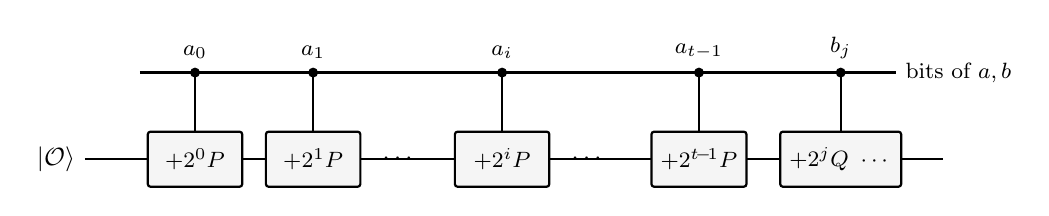
\begin{tikzpicture}[x=1cm,y=1cm,
  sm/.style={draw,thick,fill=codebg,minimum height=7mm,minimum width=12mm,rounded corners=1pt,font=\footnotesize},
]
% point wire
\draw[thick] (0,0) -- (10.9,0);
\node[left,font=\small] at (0,0) {$\lvert \mathcal{O}\rangle$};
% control rail
\draw[thick] (0.7,1.1) -- (10.3,1.1);
\node[right,font=\footnotesize] at (10.3,1.1) {bits of $a,b$};
% gate boxes
\node[sm] at (1.4,0) {$+2^0P$};
\node[sm] at (2.9,0) {$+2^1P$};
\node[font=\small] at (4.0,0) {$\cdots$};
\node[sm] at (5.3,0) {$+2^iP$};
\node[font=\small] at (6.4,0) {$\cdots$};
\node[sm] at (7.8,0) {$+2^{t\!-\!1}P$};
\node[sm] at (9.6,0) {$+2^{j}Q\ \cdots$};
% controls (dots + connectors)
\foreach \x in {1.4,2.9,5.3,7.8,9.6}{ \fill (\x,1.1) circle (1.8pt); \draw[thick] (\x,1.1) -- (\x,0.35);}
\node[above,font=\footnotesize] at (1.4,1.15) {$a_0$};
\node[above,font=\footnotesize] at (2.9,1.15) {$a_1$};
\node[above,font=\footnotesize] at (5.3,1.15) {$a_i$};
\node[above,font=\footnotesize] at (7.8,1.15) {$a_{t-1}$};
\node[above,font=\footnotesize] at (9.6,1.15) {$b_j$};
\end{tikzpicture}
\caption{Inside $U_f$ (schematic). The scalar multiplications $aP$, $bQ$ unfold via double-and-add into about $2n$ controlled point additions. Every box is the \emph{same}
point-add primitive---when its control bit is $1$, it controllably adds a \emph{classical} point to the accumulating point; the boxes differ only in "which classical point is being added" ($2^0P,2^1P,\dots,2^jQ$),
with identical circuit structure (the $i$ in $+2^iP$ stands for any bit position).}
\label{fig:oracle}
\end{figure}

\subsection{Inside point addition: why the modular inverse is the most expensive, and why it is computed twice}
\label{ssec:inv}

Return to the addition law \eqref{eq:padd} of \secref{sec:overview}: one point addition needs several $\mathbb{F}_p$ additions / subtractions / multiplications / squarings, plus \textbf{one division}
$\lambda=(y_2-y_1)(x_2-x_1)^{-1}$. The former are structurally fixed branch-free circuits, whereas that $(\cdot)^{-1}$ is a \textbf{modular inverse}
$u\mapsto u^{-1}\bmod p$, the most expensive and hardest-to-implement part of the whole circuit. This \emph{"expensive"} has a definite meaning---it contributes the most
\textbf{Toffoli gates} (and also occupies the most qubits), and the Toffoli count and qubit count are exactly the two factors of the \secref{sec:cost} score
$\text{score}=\text{Toffoli}\times\text{qubit}$. It is expensive for two reasons:

\paragraph{(a) The modular inverse is inherently data-dependent, yet must be built as an "input-oblivious" fixed-shape circuit.}
The classical algorithms for modular inverse (extended Euclid / binary GCD / Kaliski) are all \textbf{data-dependent}: the iteration count and branch decisions depend on the specific value $u$.
But a quantum circuit is a \emph{fixed unitary}---the circuit structure cannot depend on the (superposed) data (no runtime \texttt{if}), and mid-circuit measurement to decide branches
would collapse the superposition. So one can only rewrite an inherently "variable-length, branching" algorithm into an \textbf{oblivious (input-oblivious), fixed-length, fixed-shape} reversible circuit:
unfold all iterations to the worst case ($\Theta(n)$ rounds), replace \texttt{if} branches with \emph{coherent controlled swaps}, and use a fixed schedule covering all possible inputs.
This makes the modular inverse's gate count far exceed that of the other modular operations, making it the cost center of the point-add primitive.

\paragraph{(b) Reversibility demands "uncomputing" the intermediate garbage bits, nearly doubling the cost.}
A quantum circuit is unitary evolution and cannot overwrite or discard intermediate results; the large amount of scratch/ancilla produced by the modular-inverse iteration, if left untreated, would \textbf{entangle}
with the working registers and destroy the interference Shor relies on (\secref{sec:evolve}). So after each inversion, one must \emph{run the inverse of the inversion again} to cleanly
$\text{uncompute}$ the scratch back to $\lvert 0\rangle$---this is the sole reason a \emph{second} Kaliski pass runs in the circuit: besides computing the result, one must also
restore it bit-for-bit in reverse, nearly doubling the cost of point addition. (How to optimize these two parts is an engineering matter, not unpacked here.)

\subsection{The QFT circuit (why it is relatively cheap)}
\label{ssec:qft}

The $\mathrm{QFT}_M$ ($M=2^t$) of \hyperref[step:qft]{Step 3} has a standard decomposition:
\[
\mathrm{QFT}_M:\ \lvert x\rangle\longmapsto \frac{1}{\sqrt M}\sum_{y=0}^{M-1}\omega_M^{\,xy}\,\lvert y\rangle,
\]
which on the circuit is one Hadamard per wire, together with $\binom{t}{2}$ controlled phase gates $R_m=\mathrm{diag}(1,e^{2\pi i/2^m})$, for a total of
$\mathcal{O}(t^2)$ gates; dropping the exponentially small rotations (approximate QFT) lowers this to $\mathcal{O}(t\log t)$. The key point is: these are all \emph{single/two-qubit}
Clifford$+$phase gates, and compared with \hyperref[step:eval]{Step 2}'s $\Theta(n)$ point additions, each with many Toffolis, they are \textbf{negligible}. This also explains why the whole
challenge focuses only on the point-add primitive: the QFT is cheap, and what is expensive is "the reversible evaluation of $f$."

\subsection{How many qubits this circuit needs}
\label{ssec:qubits}

Qubit count (circuit width) is one of the most critical parameters of a quantum circuit, and one factor of this challenge's score $=$ (average executed Toffoli count) $\times$ (peak qubit count),
so it is worth estimating. Counting block by block per the structure above (in units of the scalar bit width $n=256$):
\begin{itemize}[leftmargin=1.4em]
\item \textbf{Two input registers}: $t\approx n$ qubits each, $\approx 2n$ total;
\item \textbf{Point accumulator}: the two $\mathbb{F}_p$ coordinates of one curve point, $\approx 2n$ total (the \emph{classical} point being added is a constant and takes no qubits);
\item \textbf{Modular-inverse / modular-arithmetic scratch}: the modular inverse (Kaliski) must maintain several $n$-bit working registers ($u,v,r,s$ and the like) simultaneously, the bulk of the width, several $n$
in all; plus carries, flags, etc.\ at $\mathcal{O}(\log n)$.
\end{itemize}
The total is $\mathcal{O}(n)$---\textbf{linear}, with no exponential $2^n$ term. To give a concrete magnitude: Roetteler--Naehrig--Svore--Lauter
(2017) estimate the \emph{entire} Shor-breaks-ECDLP circuit for secp256k1 ($n=256$) at
\[
9n+2\lceil\log_2 n\rceil+10 \;=\; 2330 \text{ logical qubits}.
\]
The coefficient $9$ is dominated by the \emph{point accumulator} ($2n$) plus the \emph{modular-inverse / field-arithmetic scratch} (several $n$), the latter the largest share; note that RNSV do \emph{not} store two full $2n$-qubit input registers---they feed the scalar bits through a \textbf{semiclassical (measure-and-recycle) QFT}, so the scalar control costs only $\mathcal{O}(1)$ qubits, not the naive $2n$ of the count above (this attribution is illustrative---check the paper for the exact per-block breakdown before citing it).

That said, this challenge does \emph{not} score this whole $2330$; it scores only the peak qubits of the \emph{single} point-add subcircuit---a subset of the machinery above. That per-primitive accounting (what the peak consists of, and why every qubit reclaimed in the modular inverse lowers the score) belongs to the implementation part---see \secref{sec:cost}.

% =====================================================================
\section{Evolution of the Quantum State}
\label{sec:evolve}
% =====================================================================

This section writes out the steps of \secref{sec:steps} as kets one by one, and \emph{rigorously} derives the readout condition \eqref{eq:readout} previewed in step four---making clear
"how the hidden period gets turned by interference into measurable peaks." For clarity, \secref{ssec:ideal} first assumes the two input registers work over $\mathbb{Z}_r$
(ideal $M=r$); \secref{ssec:leak} then returns to the real $M=2^t$ to discuss leakage.

\subsection{Preparation and reversible evaluation}

\paragraph{(1) Uniform superposition.} Each input register is prepared into a uniform superposition over $\mathbb{Z}_r$ (on a real machine this is one layer of $H^{\otimes t}$, see \secref{sec:steps}):
\begin{equation}
\lvert\psi_1\rangle=\frac{1}{r}\sum_{a=0}^{r-1}\sum_{b=0}^{r-1}\lvert a\rangle\,\lvert b\rangle\,\lvert \mathcal{O}\rangle .
\label{eq:s1}
\end{equation}

\paragraph{(2) Reversible evaluation of $f$.} Apply $U_f$ (\hyperref[step:eval]{Step 2}), writing $aP+bQ$ into the point register (using $Q=kP$, so
$aP+bQ=(a+kb)P$ is a multiple of $P$ depending only on $a+kb\bmod r$; see \eqref{eq:f}):
\begin{equation}
\lvert\psi_2\rangle=\frac{1}{r}\sum_{a,b}\lvert a\rangle\,\lvert b\rangle\,\bigl\lvert (a+kb\bmod r)\,P\bigr\rangle .
\label{eq:s2}
\end{equation}
This step evaluates $f$ over \emph{all} $r^2$ pairs $(a,b)$ at once (superposed evaluation). Note the point register's value depends only on $a+kb\bmod r$:
along $f$'s period direction $(-k,1)$, the point register's value is \textbf{many-to-one}---all $(a,b)$ connected by integer multiples of $(-k,1)$ map to the \emph{same}
point value. This is exactly the quantum version of \eqref{eq:period} (the point value is invariant along $(-k,1)$), and the physical premise for interference to work.

\subsection{Measure the value register: collapse to a coset (auxiliary viewpoint)}

The most intuitive way to analyze the interference is to imagine (without actually doing it) \emph{measuring the point register} now. Say we read the point $s_0P$, i.e.\ some
$s_0\in\mathbb{Z}_r$. By \eqref{eq:s2}, the input registers then collapse to a uniform superposition over the coset satisfying $a+kb\equiv s_0$. That coset has exactly one $a=(s_0-kb)\bmod r$
for each $b\in\mathbb{Z}_r$, $r$ terms in all, so
\begin{equation}
\lvert\psi_3\rangle=\frac{1}{\sqrt r}\sum_{b=0}^{r-1}\bigl\lvert (s_0-kb)\bmod r\bigr\rangle\,\lvert b\rangle .
\label{eq:s3}
\end{equation}
(As will be seen: \emph{not} measuring the point register gives exactly the same result---it merely tags each coset with a label that can be separated from the input registers.)

\subsection{Double QFT and the constructive-interference condition (ideal $M=r$)}
\label{ssec:ideal}

Apply $\mathrm{QFT}_r:\ \lvert x\rangle\mapsto \tfrac{1}{\sqrt r}\sum_{y}\omega_r^{xy}\lvert y\rangle$ to each input register.
Substituting \eqref{eq:s3}:
\begin{align}
\lvert\psi_4\rangle
&=\frac{1}{\sqrt r}\sum_{b}\ \Bigl(\tfrac{1}{\sqrt r}\sum_{c}\omega_r^{(s_0-kb)c}\lvert c\rangle\Bigr)
\Bigl(\tfrac{1}{\sqrt r}\sum_{d}\omega_r^{bd}\lvert d\rangle\Bigr)\notag\\
&=\frac{1}{r^{3/2}}\sum_{c,d}\ \omega_r^{s_0 c}\ \underbrace{\Bigl(\sum_{b=0}^{r-1}\omega_r^{\,b(d-kc)}\Bigr)}_{(\star)}\ \lvert c\rangle\,\lvert d\rangle .
\label{eq:s4}
\end{align}
The inner sum $(\star)$ is a complete geometric series, obeying the orthogonality relation
\begin{equation}
\sum_{b=0}^{r-1}\omega_r^{\,b(d-kc)}=
\begin{cases}
r, & d\equiv kc \pmod r,\\[2pt]
0, & \text{otherwise,}
\end{cases}
\label{eq:orth}
\end{equation}
i.e.\ only when $d\equiv kc$ do the $b$-terms align in phase and add constructively; otherwise they spread uniformly around the unit circle and cancel completely. So \eqref{eq:s4} simplifies to
\begin{equation}
\lvert\psi_4\rangle=\frac{1}{\sqrt r}\sum_{c=0}^{r-1}\omega_r^{s_0 c}\ \bigl\lvert c\bigr\rangle\,\bigl\lvert kc \bmod r\bigr\rangle .
\label{eq:s5}
\end{equation}
The measured $(c,d)$ therefore necessarily satisfies $d\equiv kc\pmod r$---exactly the readout condition \eqref{eq:readout} previewed in step four of \secref{sec:reduce},
now rigorously derived from interference. Each such $c$ appears with equal probability $1/r$; the phase $\omega_r^{s_0 c}$
affects only the phase, not the probability, so the specific value of the imagined measured $s_0$ is \emph{irrelevant}---this is exactly what "no need to actually measure the point register" means.

\subsection{Back to $M=2^t$: leakage, peak width, and rounding}
\label{ssec:leak}

A real machine uses $M=2^t$, with $b$ ranging over $\mathbb{Z}_M$, and the constraint $a\equiv s_0-kb\pmod r$ has
$\lfloor M/r\rfloor$ or $\lceil M/r\rceil$ solutions in $\mathbb{Z}_M$ for each $b$. Now the clean orthogonality of \eqref{eq:orth} no longer holds; the inner sum becomes a finite geometric series
$\sum_{m}\omega_M^{\,r m c}$, whose modulus is a \textbf{Dirichlet kernel}:
\[
\Bigl|\sum_{m=0}^{L-1}\omega_M^{\,rmc}\Bigr|
=\left|\frac{\sin(\pi\,rcL/M)}{\sin(\pi\,rc/M)}\right|,\qquad L\approx M/r,
\]
forming peaks of \emph{width about $1/M$} where $rc/M$ is near an integer, and decaying rapidly elsewhere. The two-dimensional combined conclusion is: the measured $(c,d)$ falls, with
probability $\Omega(1)$, within the $1/M$ neighborhood of some integer point $(\hat c,\hat d)$ satisfying $\hat d\equiv k\hat c\pmod r$, i.e.
\begin{equation}
\Bigl|\tfrac{c}{M}-\tfrac{\hat c}{r}\Bigr|\le\tfrac{1}{2M},\qquad
\Bigl|\tfrac{d}{M}-\tfrac{\hat d}{r}\Bigr|\le\tfrac{1}{2M}.
\label{eq:round}
\end{equation}
In other words, the only side effect of $M=2^t$ is to \emph{broaden} those clean integer points $(\hat c,\hat d)$ of \secref{ssec:ideal} into approximate rationals with $1/M$ jitter---requiring the next section's nearest-integer rounding
to exactly recover $\hat c/r,\hat d/r$, resampling if necessary. (One could also take $t$ large enough that $2^t\gtrsim r^2$, making $\hat c/r$ the \emph{unique} rational with denominator $\le r$ inside the neighborhood of \eqref{eq:round}---the continued-fraction condition of the \emph{factoring} version. But that is not needed here: because $r$ is public in ECDLP, $t\approx n$ already suffices, as \secref{sec:period} shows.)

% =====================================================================
\section{Confirming the Period}
\label{sec:period}
% =====================================================================

This is the wrap-up "after the quantum measurement," and where the private key is finally determined---but it is a \textbf{sample $\to$ classical recovery $\to$ verify} closed loop,
not a single step guaranteed to succeed at once. The emphasis on "confirming" is precisely because the quantum part only compresses the information about $k$ into one candidate \emph{with high probability},
and what truly \emph{confirms} it is that final cheap classical check.

\subsection{Recovering $k$ from $(c,d)$ (two-dimensional modular division)}

Consider the ideal case first (\secref{ssec:ideal}): measurement directly gives $(c,d)$ satisfying $d\equiv kc\pmod r$. As long as $c\not\equiv 0$, since $r$ is
prime and $c$ is invertible mod $r$,
\begin{equation}
k\;\equiv\;d\,c^{-1}\pmod r .
\label{eq:recover}
\end{equation}
One purely classical modular inverse yields the candidate $k$. The only bad sample is $c\equiv 0$ (probability $1/r$, negligible), where the formula is meaningless; discard and resample.

\paragraph{Rounding under real $M=2^t$.}\label{ssec:cf}
Real measurement gives not the clean $(\hat c,\hat d)$ but an approximation jittered by $1/M$ (\eqref{eq:round}). The key point is that in ECDLP the order $r$ is
\emph{public}: rounding $c\,r/M$ and $d\,r/M$ to the nearest integer recovers $\hat c$, $\hat d$, provided $M\gtrsim r$ (i.e.\ $t\approx n$, with rounding
error $r/2M<1/2$ guaranteeing uniqueness); substituting into \eqref{eq:recover} gives $k$. (Contrast: in the \emph{factoring} version of Shor $r$ is unknown, which is why one needs
\textbf{continued fractions} to approximate a convergent with denominator $\le r$ from $y/M$, and to take $t\gtrsim 2n$; here $r$ is known, $t\approx n$ suffices, and no continued fractions are needed.)

\subsection{Verification, failure probability, and expected number of repetitions}

Having obtained a candidate $k$, do one \textbf{cheap classical verification}: compute $kP$ (one scalar multiplication, milliseconds classically), and check
\[
kP\ \stackrel{?}{=}\ Q .
\]
\begin{itemize}[leftmargin=1.4em]
\item Equal $\Rightarrow$ the private key is recovered successfully, and the algorithm \textbf{terminates}. Because verification is deterministic, it never misjudges a wrong $k$ as correct.
\item Not equal $\Rightarrow$ this sample landed on a bad point ($c\equiv 0$, or rounding recovery failed), so go back to Step 1 of \secref{sec:steps} and resample,
until verification passes.
\end{itemize}
The probability that one quantum run gives a usable sample is a constant $\Omega(1)$ (the fraction of good $(c,d)$ times the probability $1-1/r$ that $c$ is invertible), so only
$\mathcal{O}(1)$ resamples are expected. This also shows that the algorithm's expected cost is still dominated by \hyperref[step:eval]{Step 2}'s $\Theta(n)$ reversible point additions---resampling merely multiplies it
by a constant.

\medskip
The loop thus closes: ECDLP $\xrightarrow{\text{encode}}$ the hidden period of $f$ $\xrightarrow{\text{superposed eval}+\text{QFT}}$ samples satisfying $d\equiv kc$
$\xrightarrow{\text{rounding}+\text{mod division}}$ candidate $k$ $\xrightarrow{kP\stackrel{?}{=}Q}$ confirmed private key. And the whole process's
cost is almost entirely pressed onto \hyperref[step:eval]{Step 2}, the \textbf{reversible point addition} called $\Theta(n)$ times---exactly what the \href{https://ecdsa.fail}{ecdsa.fail}
challenge optimizes. As for why this "period" exists at all, and why $f$ is chosen this way, the next section circles back to explain.

% =====================================================================
\section{Why $k$ Becomes a "Period"}
% =====================================================================

The preceding sections gave the complete mechanical flow; this section circles back to explain the \emph{intuition and design motivation} underpinning the whole construction---what is to be broken is $Q=kP$, and why $k$ would
manifest as a \emph{period} extractable by the QFT. This section introduces no new formalism and only answers "why set the problem up this way."

\paragraph{How the period is "manufactured."}
This period is not something \emph{intrinsically grown} out of $Q=kP$; rather, we deliberately choose $f(a,b)=aP+bQ$ to manufacture it. Look at when $f$ repeats
(takes the same point value):
\[
f(a,b)=f(a',b')\iff (a-a')P=(b'-b)\,Q\ \overset{Q=kP}{\Longleftrightarrow}\ a-a'\equiv k\,(b'-b)\pmod r.
\]
Taking the simplest single step---incrementing $b$ by $1$ requires decrementing $a$ by $k$ to return to the same point:
\[
f(a,b)=f(a-k,\;b+1).
\]
Why exactly $k$? Because $Q=kP$: adding one more $Q$ equals adding $k$ more $P$'s, so "$b$ takes one step" is worth "$a$ taking $k$ steps"; to keep the value unchanged,
back $a$ off by $k$ steps. This "one step of $b$ $=$ $k$ steps of $a$" holds everywhere and repeats regularly---the period arises thereby, and its ratio is exactly $k$.

\paragraph{Aside: why this attack uses $f=aP+bQ$.}
The point addition this challenge optimizes is precisely the inner building block computing this probe function $f(a,b)=aP+bQ$ (\secref{sec:circuit}). Taking $f$ as $aP+bQ$ is not arbitrary;
there are several considerations behind it, which also explain why it looks the way it does:
\begin{enumerate}[leftmargin=1.9em]
\item \textbf{It is linear (a group homomorphism).} $f$ maps $\mathbb{Z}\times\mathbb{Z}$ homomorphically into the curve group, $(1,0)\mapsto P$, $(0,1)\mapsto Q$.
Linearity makes "the $(a,b)$ that leave $f$ invariant" form exactly a \emph{subgroup / lattice}, rather than a messy set---so the period is a regular lattice, and the QFT (essentially a
Fourier transform on the group) can read it out easily; a nonlinear $f$ generally does not give such a clean period.
\item \textbf{It uses both $P$ and $Q$ at once.} $k$ hides in the \emph{coupling} of the two: looking at a single axis, the periods of $f(a,0)=aP$ and $f(0,b)=bQ$ are both the
\emph{public} $r$; it is "adding $aP$ and $bQ$," borrowing $Q=kP$, that ties the two axes together at ratio $k$, so that $k$ shows up as a slope. This is also why it has one more dimension than the factoring
version.
\item \textbf{It can be computed efficiently and reversibly.} $aP+bQ$ can be realized reversibly in $\mathrm{poly}(n)$ gates via double-and-add ($U_f$)---this is the practical
threshold for whether it can actually run on a quantum machine.
\item \textbf{It satisfies the "hiding" condition.} $f(a,b)=(a+kb\bmod r)P$ takes the same value on the same line $a+kb\equiv$constant and \emph{different}
values on different lines (corresponding to $r$ distinct points), so the period is "clean" and can be read out unambiguously---exactly the hiding property the abelian hidden subgroup problem requires.
\end{enumerate}
The natural landing point satisfying these is $f=aP+bQ$.

% #####################################################################
\part{Implementation: What the ecdsafail-challenge Actually Does}
% #####################################################################

Part~I covered the \emph{general} algorithmic principle; this part maps it onto the actual secp256k1 point-add challenge source: which segment the challenge actually implements,
and which file / function each section of Part~I lands in. (Paths below are relative to the ecdsafail-challenge repo root; line numbers drift with refactoring, so only file and function names are given.)

% =====================================================================
\section{Which segment this challenge actually implements}
\label{sec:target}
% =====================================================================

The challenge implements only the \textbf{single point addition} primitive: given a quantum point target $(x,y)$ (qubits) and a classical point offset $(x,y)$ (classical
bits), reversibly overwrite target \emph{in place} with the affine sum $\text{target}+\text{offset}$ (on secp256k1). It does not include the QFT,
measurement, the whole $aP+bQ$, and has no $a,b$ input registers---these are the \emph{algorithm layer} of Part~I ("why it is done this way"), which have no code entity here;
what the challenge corresponds to is only the innermost \emph{single point-add step} (Part~I's Step 2, \secref{sec:circuit}).

\paragraph{Why single out just this segment.}
The most direct reason is that it can be \emph{classically} verified: a single point addition is a reversible \emph{classical permutation}, checkable point by point on an ordinary machine against 9024 test points; whereas
the full Shor with QFT / true superposition either cannot be classically simulated or requires a real quantum machine (which would already amount to a real break)---point addition is the largest chunk that "can still be checked on a laptop."
As for the other reasons---it is the \emph{bottleneck} of the whole attack, amplified $\approx 2n$ times as the innermost loop, and the only component still with algorithmic
freedom left---those are exactly the themes to be unpacked in \secref{sec:cost} and \secref{sec:gcd}.

\paragraph{Interface and scoring (the contract).}The circuit must consume four 256-element registers---\code{target_x}, \code{target_y} (qubits) and
\code{offset_x}, \code{offset_y} (classical bits)---and overwrite \code{target_x}, \code{target_y} \emph{in place} with the
affine sum. The scoring is consistent with Part~I's "why press Toffoli$\times$qubit": $\text{score}=\overline{\text{Toffoli}}\times$peak qubits,
\emph{lower is better} (the industrial meaning of this metric is in \secref{sec:cost}).

\paragraph{What counts as "valid": the $0/0/0$ conditions.}A submission must pass on all 9024 test points; failing any single one means a loss. The name "$0/0/0$" refers to the three error channels---classical, phase, and ancilla---all reading zero; concretely this unpacks into the following checks:
\begin{enumerate}[leftmargin=1.9em]
\item \textbf{Classically correct.} All 9024 points must compute the correct $(R_x,R_y)$.
\item \textbf{Reversible (ancilla zeroed).} Every ancilla must be uncomputed back to $|0\rangle$ before release; after the forward pass, all non-output qubits must also return to $|0\rangle$.
\item \textbf{Phase-clean.} The global phase of all surviving branches is zero---no phase kickback left by incomplete uncomputation.
\item \textbf{Forward$\circ$inverse identity.} Running the circuit once and then its gate-level inverse must restore the initial state qubit by qubit.
\end{enumerate}
These four conditions block all "fake wins": any drop in Toffoli count bought by skipping uncomputation, leaking phase, or dumping garbage into ancilla only makes this submission \emph{lose} rather than run faster.
The reason "reversible + phase-clean" is enforced even for a primitive verified only on \emph{classical} points is that it will eventually be embedded in a real Shor, acting on a \emph{superposition}
(\secref{sec:circuit}): then unzeroed ancilla and residual phase would pollute the interference and destroy the whole attack---these two conditions are exactly the threshold that upgrades "classically correct" to "quantum-usable."

\paragraph{What can and cannot be changed, and why.}
\begin{itemize}[leftmargin=1.4em]
\item \textbf{Changeable:} everything in \code{src/point_add/}---split modules, rewrite the primitive, swap algorithms, refactor freely. All the optimization space is here.
\item \textbf{The unchangeable "contract layer":} the harness---\code{src/lib.rs}, \code{circuit.rs}, \code{sim.rs},
\code{weierstrass_elliptic_curve.rs}, and the \code{src/bin/} drivers---which defines the interface, the counting rules (counting every Toffoli / Clifford / peak qubit), the $0/0/0$ checks, and the scoring;
plus \code{Cargo.toml} / \code{Cargo.lock} / \code{rust-toolchain} (no new dependencies allowed), and no writing directly to \code{results.tsv}.
\end{itemize}
The design intent is plain: \emph{separate the referee from the player}. If the counting, checking, and reference curve could be changed, one could cheat by changing "how it counts," and the score would lose meaning; locking down the harness
guarantees the score reflects only \emph{the algorithm itself} and that different submissions are comparable. The test points are derived by \textbf{Fiat--Shamir} hashing of the submitted op stream, so players cannot tune to the test set
(cannot "memorize" the circuit to work only on fixed point pairs); the no-new-dependencies rule works the same way, preventing cost from being outsourced to a library. So the only way to lower the score is to genuinely make that modular inverse
of \secref{sec:gcd} cheaper---which is exactly what the competition is designed to force out.

% =====================================================================
\section{Why industry wants to minimize Toffoli count $\times$ qubit count}
\label{sec:cost}
% =====================================================================

\secref{sec:target} already gave the scoring scalar $\text{score}=\overline{\text{Toffoli}}\times$peak qubits (lower is better); this section clarifies its
\emph{industrial motivation}---why the metric of greatest concern is exactly the \textbf{product of executed Toffoli gates and occupied qubits}, and not the total gate count or anything else.

\paragraph{First, pin down which step this score measures.}
Back to \secref{sec:steps} and \secref{ssec:qft}: across the whole algorithm, preparing the superposition (one layer of $H$) and the two QFTs are only cheap single/two-qubit
gates, so almost all Toffolis come from \hyperref[step:eval]{Step 2}'s reversible evaluation $U_f$, and the circuit's peak qubits are also reached during $U_f$ (those wide
modular-inverse scratch registers). So the two quantities in the score---executed Toffoli count and peak qubits---essentially measure \hyperref[step:eval]{Step 2},
more precisely the execution cost of its innermost \textbf{point-add primitive}, called repeatedly by double-and-add. In a word: \emph{scoring the resources of the whole Shor
attack is roughly scoring this one point-add primitive}---Steps 1 and 3 barely count.

\paragraph{What the scored peak actually is (and how big).}
Concretely, the scored peak is that single point-add subcircuit's own footprint: \emph{point accumulator} ($\approx2n$) $+$ \emph{modular-inverse scratch} (several $n$), reaching its high-water mark
during the modular-inverse phase (\secref{ssec:inv}), and \textbf{excluding} the two $2n$ input registers (they belong to the \emph{outer} double-and-add loop, and do not enter a \emph{single} point
addition). So it is a strict \emph{subset} of the machinery counted in the $2330$ of \secref{ssec:qubits}---magnitude $\sim 4.5n$ (currently measured at a frontier peak of $\approx 1150$
qubits), \emph{not} "$2330$ minus the input registers." Because the score is $\overline{\text{Toffoli}}\times$peak qubits, every qubit reclaimed in the modular inverse directly lowers
the score, exactly as it lowers the Toffoli factor---which is why \secref{sec:gcd} treats the modular inverse as the joint cost center of both factors.

\paragraph{So why measure it as "the two multiplied together"?}
Because this product is a clean proxy for the \textbf{space--time volume of fault-tolerant quantum computing (FTQC)}, and space--time volume is the real
physical cost:

\begin{itemize}[leftmargin=1.4em]
\item \textbf{Toffoli / T gates are the only expensive gates (the time axis).} Under mainstream error-correcting architectures like the surface code, Clifford gates are nearly free, whereas every
Toffoli (or T gate) must be supplied by \emph{magic state distillation}---distillation factories occupy the vast majority of a fault-tolerant machine's physical
cost and runtime. So "average executed Toffoli count" is directly proportional to the distillation load, roughly the \emph{runtime} of this computation.
\item \textbf{Peak qubit count determines how big the machine must be (the space axis).} Each logical qubit costs thousands of physical qubits under error correction; the peak
width determines "how wide the machine must at least be," roughly the machine's \emph{scale}.
\item \textbf{The product of the two $=$ space--time volume.} Multiplying "runtime" by "machine scale" gives the space--time resources this computation occupies on a fault-tolerant machine---the
real cost and engineering effort.
\end{itemize}

Now layer on the amplification effect stressed repeatedly here: point addition is called $\Theta(n)$ ($n=256$) times in one complete Shor attack (the
double-and-add of \eqref{eq:dbladd}), so any constant-factor reduction on a single point addition multiplies by several hundred along the whole algorithm. The number industry really cares about---"how big a fault-tolerant machine
and how many hours it takes to break secp256k1 with a quantum computer"---is proportional to this amplified space--time volume; pressing down the point addition's
$\text{Toffoli}\times\text{qubit}$ is equivalent to \emph{directly revising down} this threat estimate.

\paragraph{The full-attack cost, concretely.}
The state-of-the-art resource estimates\footnote{Google Quantum AI et al.\ (2026), \url{https://arxiv.org/abs/2603.28846}; the windowing accounting and \eqref{eq:fullcost} are its Appendix~A, Eq.~(A1), p.~55. (Exact citation to confirm.) See also D.~Litinski, \emph{How to compute a 256-bit elliptic curve private key with only 50 million Toffoli gates} (2023), \url{https://arxiv.org/abs/2306.08585}, for a clear exposition of this windowing accounting.} use \emph{windowed} additions rather than the plain double-and-add of \eqref{eq:dbladd}: $w$ consecutive additions are merged into one, at the cost of a size-$2^{w}$ table lookup ($3\cdot2^{w}$ Toffoli) with the added point selected coherently from a precomputed table. The total non-Clifford (Toffoli) cost of the whole $n$-bit ECDLP circuit is then
\begin{equation}
\mathrm{ECDLP}^{\mathrm{Toff}}_n=\bigl(\mathrm{PA}^{\mathrm{Toff}}_n+3\cdot2^{w}\bigr)\Bigl(\tfrac{2n}{w}-4\Bigr),
\label{eq:fullcost}
\end{equation}
where $\mathrm{PA}^{\mathrm{Toff}}_n$ is the Toffoli count of one point-addition core (the quantity this challenge optimizes) and the $-4$ absorbs two standard end-of-schedule savings (replacing the first windowed addition by a direct lookup, and skipping the last three by classical post-processing). For $n=256$, $w=16$ this is $28\times(3\cdot2^{16}+\mathrm{PA}^{\mathrm{Toff}}_{256})$, with $2n/w-4=32-4=28$ windowed additions. So lowering the scored per-addition cost feeds \emph{directly} into this full-attack total. (Reconciling the challenge's classical-offset primitive with the windowed, coherently-selected point---and the apples-to-apples comparison against those estimates---is carried out in the companion writeup, not here.)

And this estimate is precisely the quantitative basis for the NIST post-quantum
standardization process and for the ECDSA-deprecation timelines in finance / blockchain / TLS and other industries.

% =====================================================================
\section{Why the main battlefield of optimization is the GCD (modular inverse)}
\label{sec:gcd}
% =====================================================================

The previous section explained \emph{what to press}---the space--time volume $\text{Toffoli}\times\text{qubit}$; this section explains \emph{where to press}. The answer is highly
concentrated: the \textbf{modular inverse} inside point addition, i.e.\ the step computed by binary GCD / Kaliski (\secref{ssec:inv}). One might say
much of the optimization history of this circuit has been the optimization history of the modular inverse (GCD)---though, as noted below, the surrounding field arithmetic still yields wins too. There are four reasons the GCD dominates, and they compound:

\paragraph{(1) It is the only iterative big-cost component in point addition.}
In one point addition (\eqref{eq:padd}), addition / subtraction / multiplication / squaring are all \emph{branch-free, single-pass} circuits with fixed structure, and the adder (Gidney-style) and
schoolbook / Karatsuba multiplication are already heavily optimized (though \emph{not} provably minimal---the field arithmetic still yields the occasional win, see the end of the section). Only the modular inverse has \emph{no} single-pass algorithm; it can only iterate GCD for
$\Theta(n)$ (about $256$--$512$) rounds, each round a compare $+$ conditional subtract $+$ shift. One multiplication is one pass, GCD is $n$ passes---so
the Toffolis of a single point addition come mainly from the GCD loop body.

\paragraph{(2) It maxes out both factors of the score at once.}
The score is a \emph{product} $\text{Toffoli}\times\text{qubit}$, so the component that can lower both factors yields the most, and the GCD occupies both:
\begin{itemize}[leftmargin=1.4em]
\item \textbf{Toffoli axis}: $\Theta(n)$ rounds $\times$ the comparator / conditional subtraction per round, the bulk of the point addition's gate count.
\item \textbf{Qubit axis}: Kaliski must maintain several $n$-bit state registers ($u,v,r,s$ and the like) plus scratch at once, and the peak width of the whole
circuit is often reached during the GCD phase.
\end{itemize}
Other components usually improve only one factor; the GCD is one of the few that \emph{affects both factors at once}, with the largest marginal gain on the product.

\paragraph{(3) Reversibility doubles it, double-and-add amplifies it.}
The scratch produced by the modular inverse must be uncomputed to zero (the second Kaliski pass, \secref{ssec:inv}), so saving one share on the GCD actually saves two;
and the modular inverse is called once per point addition, and point addition is called $\Theta(n)$ times by double-and-add (\eqref{eq:dbladd}), so any constant
factor pressed down here multiplies by several hundred along the whole algorithm. Savings on other components are additive; savings on the GCD are multiplicative.

\paragraph{(4) It has the most algorithmic freedom left.}
The adder / multiplication / squaring are structurally fixed single-pass circuits, already close to their practical limits---so the place in one point addition where the \emph{biggest} trade-offs remain---\emph{which modular-inverse
algorithm to choose and how to organize its iterations}---is concentrated in the GCD, which is still an open design problem. This does not mean the field arithmetic is frozen: it is heavily optimized but not provably minimal, and recent frontier moves have still come from restructuring it---for instance, rewriting the modular \emph{squaring} from an AND-based schoolbook form into a controlled add--subtract (roughly halving the Toffolis per cross product) delivered a few-percent score improvement without touching the GCD. But such wins are the exception; the largest and most reliable leverage is still the modular inverse, and focusing on it is not a preference but what the circuit structure dictates.

\medskip
In a word: minimizing $\text{Toffoli}\times\text{qubit}$ is, to first order, reducing the cost of the modular inverse---the GCD is the largest cost
center, the amplifier, and the richest locus of algorithmic freedom of a single point addition, with the surrounding field arithmetic a secondary lever. This is also why, on this circuit, most advances that push cost to a new low ultimately trace back to the same place:
lowering the cost of that one modular-inverse step.

% =====================================================================
\section{Where the code is: peeling inward along point addition}
% =====================================================================

Peeling inward along "a single point addition," the code has roughly four layers, each more of an optimization focus the deeper it goes:

\begin{itemize}[leftmargin=1.4em]
\item \textbf{Top-level point addition} --- \code{ec_add()} in \code{src/point_add/trailmix_ludicrous/ec_add.rs} (entry
\code{point_add/mod.rs::build()}). It adds a classical point in place to the quantum point, using exactly Part~I's addition law \eqref{eq:padd} for
$\lambda,x_3,y_3$ (the file header comment is "a-independent secp add formula," just optimized in place).
\item \textbf{The most expensive part---the modular inverse} --- \code{gcd.rs}, the jump-GCD for $y\mapsto y\cdot x^{-1}\bmod q$ (here $q=p$ is the field prime---the code's variable name for it; not the group order $r$). This is the entity referred to by \secref{ssec:inv}'s
"most expensive, computed twice" and \secref{sec:gcd}'s "the GCD is the cost center," and the file actually optimized over and over; the schedule /
comparator / venting / constant-propagation machinery around it is in \code{schedule.rs}, \code{comparator.rs}, \code{venting.rs}, and \code{constprop.rs}.
\item \textbf{The rest of the arithmetic} (modular multiplication / squaring / addition / comparison --- heavily optimized, though still an occasional source of wins, e.g.\ a recent restructuring of the modular squaring) --- \code{src/point_add/arith/} and \code{gidney.rs},
\code{multiply.rs}, \code{square.rs}.
\item \textbf{Verification and scoring} --- \code{src/sim.rs} runs $0/0/0$ on the 9024 test points and counts Toffolis and peak qubits;
\code{src/bin/eval_circuit.rs} sets the secp256k1 parameters, computes the reference point addition, and scores $\overline{\text{Toffoli}}\times$peak qubits
(\secref{sec:cost}). The curve's classical reference is in \code{src/weierstrass_elliptic_curve.rs}.
\end{itemize}

In a word: the whole codebase is the implementation of Part~I's innermost "single point-add step," and the deeper in (the modular inverse / GCD), the more it is the optimization battlefield.

\end{document}
